\section{Conceptos básicos de hidráulica urbana en RDA}
Conjunto de elementos enlazados de tal manera que permite suministrar cierta cantidad de agua a una presión establecida~\cite{Doctoral2012}.

\paragraph{Presion:} Fuerza ejercida sobre una superficie.
\paragraph{Caudal:} Cantidad de agua que se mueve a través de un segmento de la red.
\paragraph{Factor de fricción:} Coeficiente adimensional que especifica la rugosidad de la tubería~\cite{Perez-2011}.
\paragraph{Curva de consumo:}

\subsection{Componentes físicos de una red}
A continuación se define los componentes que conforman una red de agua potable~\cite{Rossman2017}, los cuales se aprecian en la Figura~\ref{fig:componentesfisicos}:


\begin{figure}[h]
	 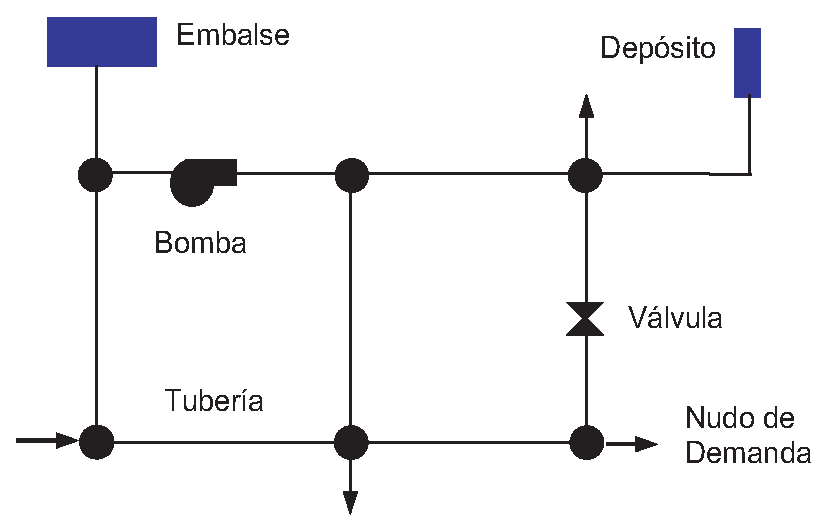
\includegraphics{Capitulo2/assets/componentesfisicosred.eps}
	\centering
	\caption[Componentes físicos de un sistema de distribución de agua]{Componentes físicos de un sistema de distribución de agua~\cite{Rossman2017}}
	\label{fig:componentesfisicos}
\end{figure}
\paragraph{Nudos de consumo:} Son los puntos o extremos de una tubería, los cuales también permiten que estas se unan. Estos nudos pueden actuar como nudos de demanda a través de los cuales el flujo abandona la red.

\paragraph{Reservorio:}Es una fuente de alimentación externa.
\paragraph{Deposito:}Son elementos con la capacidad de almacenar agua.
\paragraph{Tuberias:}Son los elementos a través de los cuales transita el agua de un nudo a otro.
\paragraph{Bombas:}Elementos que permiten impulsar el liquido con el fin de elevarlo a una posición superior.
\paragraph{Válvulas:}Elementos que limitan la presión o el caudal que transita en un punto de la red.